\documentclass[sigconf,screen,review]{acmart}

\setcopyright{none}
\settopmatter{printacmref=false, printccs=false, printfolios=true}
\renewcommand\footnotetextcopyrightpermission[1]{}
\pagestyle{plain}

\usepackage{booktabs}
\usepackage{array}
\usepackage{enumitem}
\usepackage{xcolor}
\usepackage{balance}

\setlist[itemize]{leftmargin=1.2em}
\setlist[enumerate]{leftmargin=1.4em}
\renewcommand{\arraystretch}{1.08}

\title{Weekly Report}
\subtitle{Week of June 10, 2026}

\begin{document}

\maketitle

\section{Data Path Optimization}

\subsection{Experiment Setup}

This week's experiments focus on two related questions.

\textbf{Data path breakdown.}  I designed a fine-grained L1V data-path
breakdown that starts from the L1V cache entry point and follows each selected
coalesced L1V cache-line request until the response returns to L1V
(Figure~\ref{fig:l1v-data-path}).  Each run collects 100K selected L1V paths
and exits after the trace window is complete.  This breakdown showed that
\texttt{AT -> L1V}, the time before a translated vector-memory request can
enter L1V, was a major bottleneck.  To test whether this was an L1V admission
limit, I created a ``super L1V'' configuration by increasing the L1V MSHR
capacity and maximum concurrent L1V transactions to 160 entries each
(160-MSHR/160-concurrency).

The data-path experiment compares two traditional-workload runs with the same
L1V path trace mode enabled.  These two runs use the corrected lower L1V bank
latency, after the earlier 60-cycle L1V bank latency was found to overstate the
L1V hit path.

\begin{itemize}
  \item Baseline L1V configuration: default 16 MSHR entries and 16 maximum
  concurrent transactions.
  \item New L1V configuration: 160 MSHR entries and 160 maximum concurrent
  transactions.
\end{itemize}

Both runs completed the same 13 traditional workloads with L1V path summaries.

\section{Main Observation}

The new configuration removes the previous L1V admission bottleneck.  In many
workloads, \texttt{AT -> L1V} falls from tens or hundreds of ns to about 1 ns.
This means the earlier \texttt{AT -> L1V} term was not simply address
translation latency.  It was largely admission/backpressure before the request
could be accepted by the L1V cache/coalescer.

However, removing that admission bottleneck does not automatically improve
performance.  Matrix multiplication is the clearest case.  Its average L1V
path latency increases from 492 ns to 1693 ns, while \texttt{AT -> L1V} drops
from 214 ns to 1.01 ns.  The bottleneck has moved downstream.

Figure~\ref{fig:l1v-data-path} shows the traced data path.  The route is
selected at the L1V miss point.  A local miss goes to the local L2 and then to
local DRAM on an L2 miss.  A remote miss goes through local RDMA, remote RDMA,
remote L2, and remote DRAM only if the remote L2 misses.

\begin{figure*}[t]
  \centering
  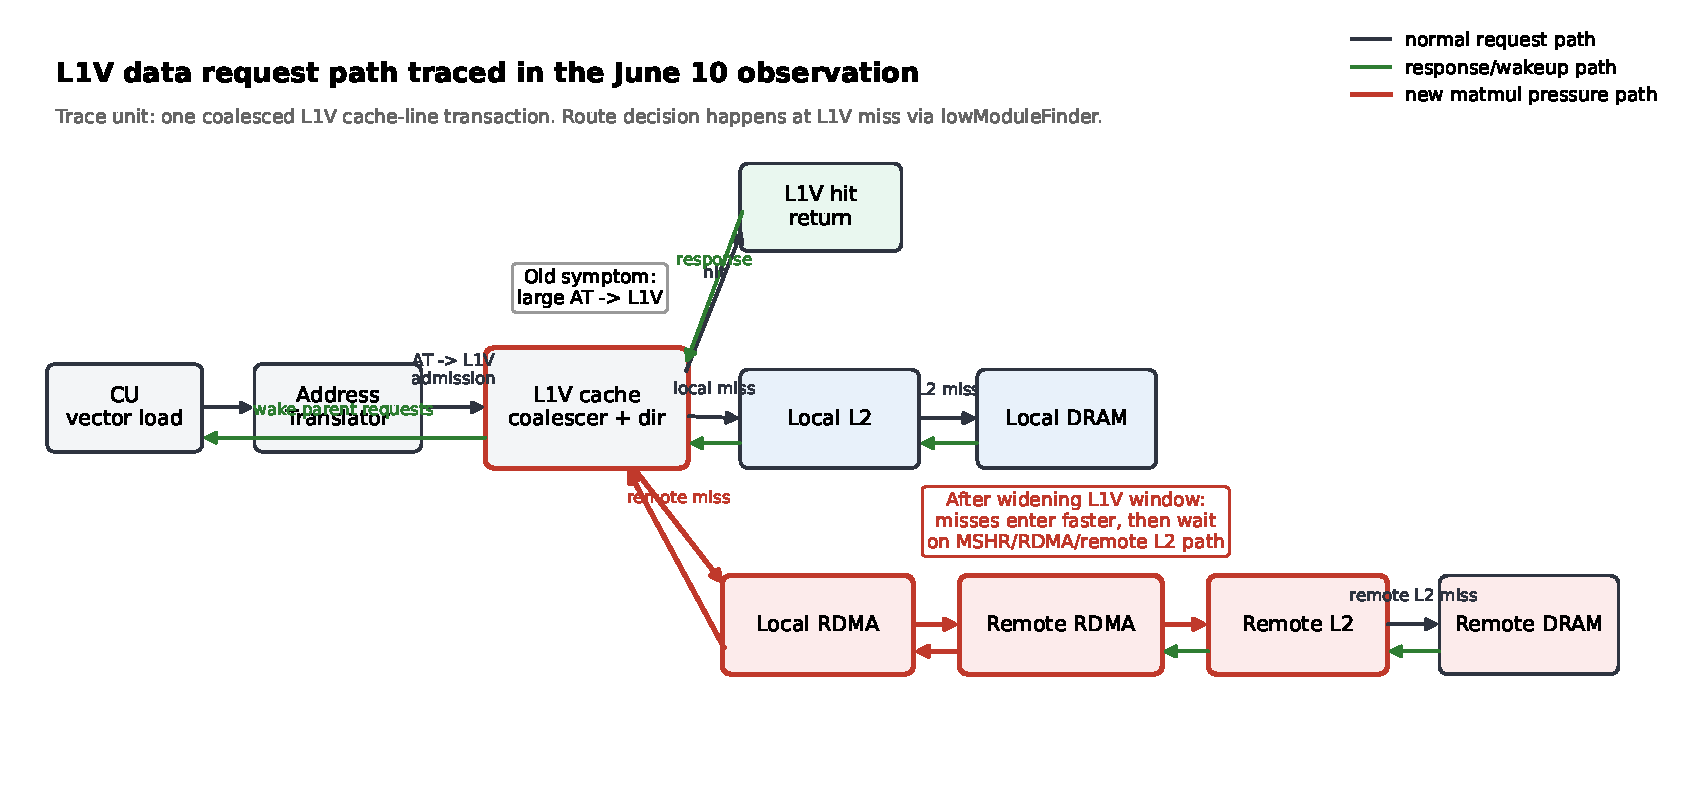
\includegraphics[width=0.98\textwidth]{figures/l1v_data_path.pdf}
  \caption{L1V request data path used by the fine-grained trace.  The old
  pressure appeared before L1V admission.  After increasing the L1V MSHR and
  concurrent transaction window, matrix multiplication shifts pressure to the
  L1V miss-completion path, especially MSHR waiting, the cross-GPU request
  transfer, and the cross-GPU data-return transfer.}
  \label{fig:l1v-data-path}
\end{figure*}

\begin{table*}[t]
  \centering
  \caption{L1V path comparison before and after increasing both L1V MSHR
  entries and maximum concurrent L1V transactions to 160.  Latencies are
  average ns per selected L1V path.}
  \label{tab:l1v-path-comparison}
  \begin{tabular}{lrrrrrr}
    \toprule
    Workload & Old total & New total & Change &
    Old AT$\rightarrow$L1V & New AT$\rightarrow$L1V &
    New remote \% \\
    \midrule
    AES & 127.48 & 226.19 & +77.4\% & 48.93 & 1.00 & 0.0 \\
    BitonicSort & 232.41 & 260.80 & +12.2\% & 80.33 & 1.00 & 51.5 \\
    FWT & 84.90 & 115.04 & +35.5\% & 25.75 & 1.00 & 0.3 \\
    FFT & 152.30 & 308.16 & +102.3\% & 85.57 & 1.06 & 0.0 \\
    FIR & 101.87 & 102.82 & +0.9\% & 4.81 & 1.00 & 25.2 \\
    FloydWarshall & 104.46 & 113.26 & +8.4\% & 15.00 & 6.73 & 6.6 \\
    Im2Col & 294.85 & 302.26 & +2.5\% & 7.92 & 1.57 & 89.9 \\
    KMeans & 118.46 & 127.32 & +7.5\% & 12.97 & 1.00 & 7.7 \\
    MatMul & 491.63 & 1693.07 & +244.4\% & 214.22 & 1.01 & 17.2 \\
    MatMul-MiddleTile & 488.55 & 881.38 & +80.4\% & 221.82 & 5.57 & 14.2 \\
    PageRank & 66.13 & 69.24 & +4.7\% & 6.28 & 1.00 & 6.1 \\
    SpMV & 65.06 & 95.10 & +46.2\% & 30.96 & 1.00 & 0.0 \\
    Stencil2D & 355.43 & 355.36 & -0.0\% & 1.00 & 1.00 & 79.8 \\
    \bottomrule
  \end{tabular}
\end{table*}

\begin{figure*}[t]
  \centering
  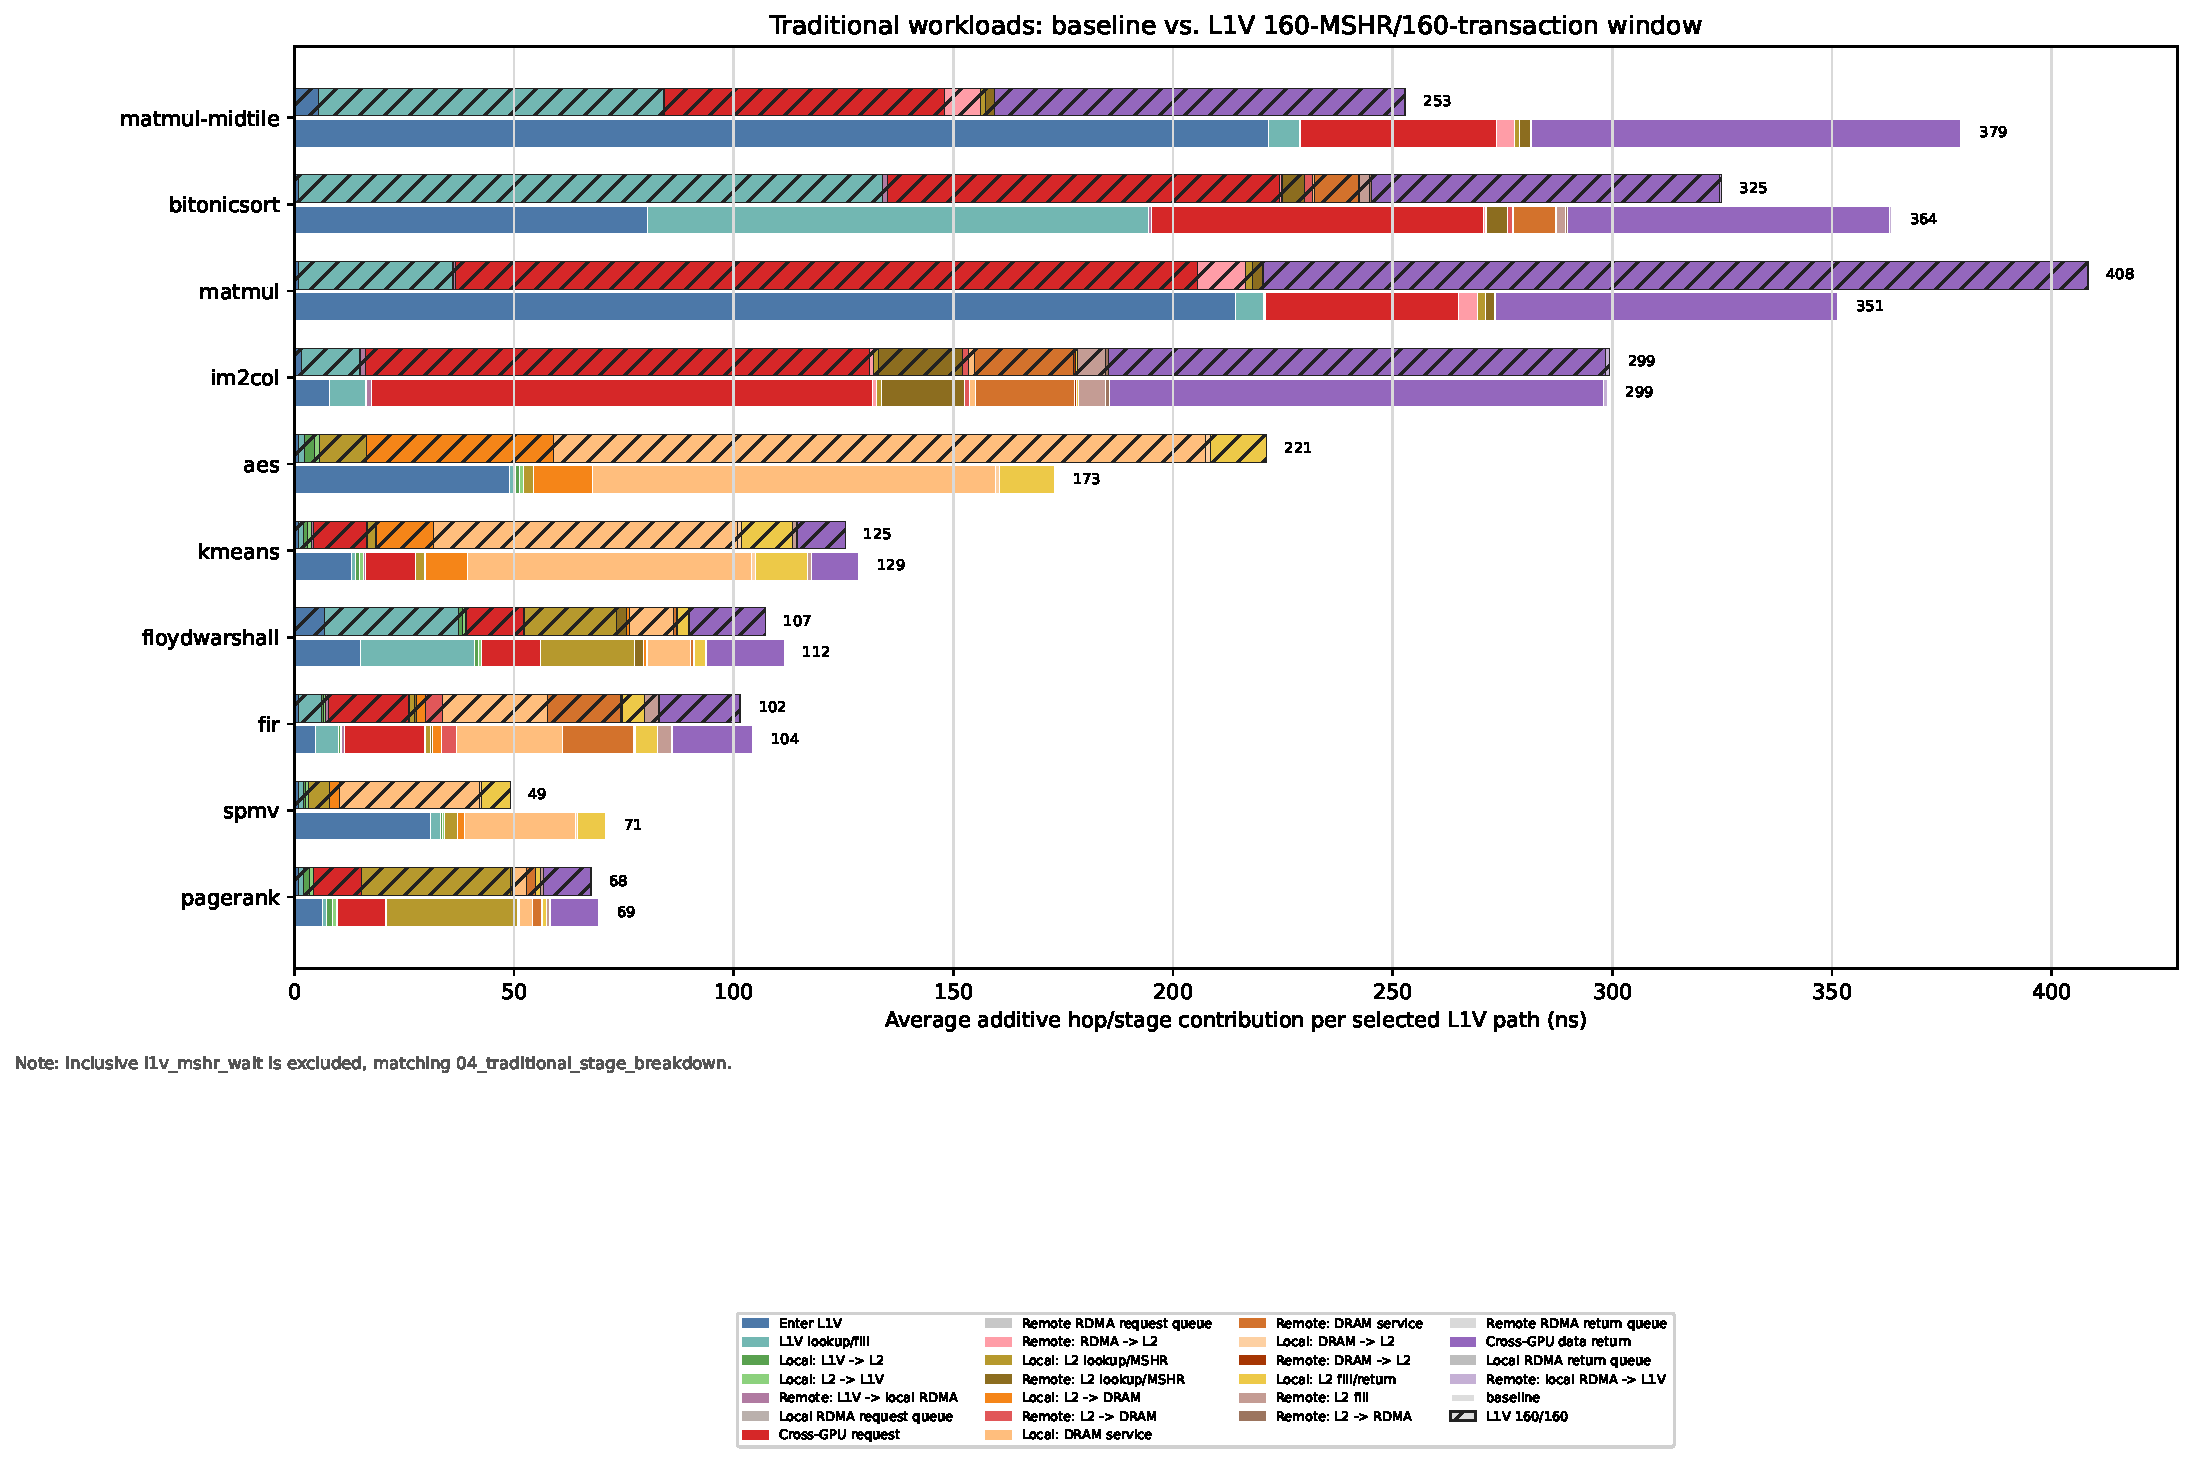
\includegraphics[width=0.98\textwidth]{figures/traditional_stage_breakdown_baseline_vs_l1v160_rdma_expanded_plainnames.pdf}
  \caption{Traditional workload additive L1V stage breakdown, comparing the
  baseline run against the 160-MSHR/160-transaction L1V configuration, with
  remote request and return paths expanded.  Solid bars are baseline; hatched
  bars are the wider L1V configuration.  Here \texttt{Cross-GPU request} means
  the local-RDMA to remote-RDMA request transfer, and
  \texttt{Cross-GPU data return} means only the remote-RDMA to local-RDMA data
  transfer.  Local and remote L2/DRAM stages are separated using each traced
  path's route field.  Remote-RDMA to L2, L2 to DRAM, DRAM service, DRAM to
  L2, and L2 to RDMA are shown as separate stages.  Inclusive
  \texttt{l1v\_mshr\_wait} is excluded to avoid double-counting lower-path
  hops.}
  \label{fig:traditional-stage-compare}
\end{figure*}

\section{Matrix Multiplication Case Study}

Matrix multiplication is the important negative result.  After increasing L1V
MSHR and transaction capacity, \texttt{AT -> L1V} is almost eliminated, but
the run gets slower.

\begin{table}[t]
  \centering
  \caption{Matrix multiplication stage movement.  The old run is the default
  L1V configuration; the new run uses 160 MSHRs and 160 concurrent
  transactions.}
  \label{tab:matmul-stage}
  \begin{tabular}{lrrr}
    \toprule
    Metric & Old & New & Change \\
    \midrule
    Total L1V path latency & 491.63 & 1693.07 & +244.4\% \\
    \texttt{AT -> L1V} & 214.22 & 1.01 & -99.5\% \\
    \texttt{l1v\_dir\_lookup} & 2.59 & 33.20 & +1181.6\% \\
    \texttt{l1v\_mshr\_wait} & 131.00 & 372.59 & +184.4\% \\
    Cross-GPU request transfer & 43.8 & 169.0 & +285.8\% \\
    Cross-GPU data-return transfer & 77.9 & 187.6 & +140.9\% \\
    Driver total time & 4.879 us & 7.834 us & +60.6\% \\
    \bottomrule
  \end{tabular}
\end{table}

The \texttt{mshr-hit} population also changes substantially.  In the old run,
48,272 out of 100K selected paths were L1V MSHR hits, with an average path
latency of 735 ns.  In the new run, 64,360 paths are MSHR hits, with an
average path latency of 2023 ns.  This means that the wider L1V front end lets
many more requests enter the cache hierarchy, but a larger fraction of them
wait behind outstanding misses.

\section{Interpretation}

The key interpretation is:

\begin{quote}
Before the change, matrix multiplication was bottlenecked at L1V admission.
After the change, requests enter L1V easily, but the latency center shifts to
the L1V miss path: MSHR waiting, the cross-GPU request transfer, the
cross-GPU data-return transfer, and remote L2 service.
\end{quote}

This suggests that the old \texttt{AT -> L1V} pressure was partly acting as a
throttle.  It limited how many misses could be injected into the downstream
memory system.  Once that throttle is removed, matrix multiplication exposes a
deeper remote-path bottleneck.

This also explains why the result is workload-dependent.  Some workloads
benefit in the 100K-path completion time:

\begin{itemize}
  \item BitonicSort improves from 6.723 us to 5.833 us.
  \item FIR improves from 3.706 us to 3.664 us.
  \item PageRank improves from 6.177 us to 6.079 us.
\end{itemize}

But regular matrix multiplication becomes worse, from 4.879 us to 7.834 us.
Therefore, simply increasing L1V MSHR capacity is not a universally good
optimization.  It can expose or amplify downstream contention.

\section{Design Implications}

The current evidence points to three design implications.

\textbf{First, L1V admission and L1V path completion must be separated.}
\texttt{AT -> L1V} is an entry-side symptom.  It can be removed by widening the
L1V transaction window, but that does not mean the memory hierarchy is faster.

\textbf{Second, matrix multiplication is not primarily fixed by larger L1V
MSHRs.}  Once enough requests enter L1V, the dominant cost is waiting for
remote or lower-level service to complete.  The important path is:

The important path is: L1V miss to local RDMA, remote RDMA, remote L2, and
then the response path back to L1V.

\textbf{Third, future mechanisms need either controlled injection or faster
remote service.}  Possible next steps include separate local/remote MSHR
quotas, adaptive L1V admission, larger RDMA queues/bandwidth, or a neighbor-L2
design that gives remote requesters a lower-latency cache path without
interfering too much with local traffic.

\section{Per-GPU Imbalance Observation}

The Photon/sampled-simulation debugging exposed a second, separate issue:
matrix multiplication shows strong spatial imbalance across the 7-by-7
wafer layout.  This imbalance is visible even without Photon prediction.  A
clean no-predict matrix multiplication run with the same endpoint/network
settings reached a state where normal GPU tiles ranged from 8\% to 64\%
completed workgroup progress.  The corresponding
\texttt{sample\_all\_w512\_g512} run ranged from 14\% to 58\%, but that run
was externally terminated before completion.  Therefore the current evidence
does not support blaming Photon prediction alone; the detailed WSG execution
already contains a spatial straggler pattern.

The completed sampled run gives the same type of signal from final per-GPU
\texttt{CommandProcessor} kernel time.  That run used
\texttt{sample\_all\_loop\_w128\_g512}; it is useful for finding imbalance
patterns, but it should not be treated as strict Photon because loop sampling
is a local extension.  In this completed result, regular matrix multiplication
has a 9.29$\times$ max/min spread, while the middle-tile matrix multiplication
variant has a 19.26$\times$ max/min spread.  The middle-tile case is dominated
by tile 42, which reaches 28.02 ms while the median tile is only 3.17 ms.

\begin{table}[t]
  \centering
  \caption{Benchmarks with the strongest completed per-GPU kernel-time
  imbalance in the sampled result set.  The ranking uses max/median rather
  than max/min, because a very small minimum tile can exaggerate max/min.}
  \label{tab:gpu-imbalance-benchmarks}
  \begin{tabular}{lrrl}
    \toprule
    Benchmark & Max/Med & Max/Min & Slowest tiles \\
    \midrule
    MatMul-MiddleTile & 8.83 & 19.26 & T42, T46, T25 \\
    AES & 8.19 & 9.29 & T41, T2, T31 \\
    MatMul & 2.92 & 9.29 & T14, T34, T19 \\
    BitonicSort & 2.34 & 2.91 & T28, T27, T13 \\
    FIR & 1.49 & 12.33 & T18, T16, T19 \\
    FWT & 1.34 & 5.76 & T44, T37, T43 \\
    Stencil2D & 1.23 & 2.05 & T20, T30, T27 \\
    KMeans & 1.23 & 2.49 & T20, T28, T7 \\
    \bottomrule
  \end{tabular}
\end{table}

FFT, Im2Col, PageRank, SpMV, and FloydWarshall are comparatively balanced in
the same result set.

\section{Next Experiments}

The next experiments should avoid changing only one limit in isolation.  A
useful sweep would be:

\begin{enumerate}
  \item Keep the 160-entry MSHR and 160-transaction window, then increase the
  number of L1V requests processed per cycle to 8.
  \item Increase L1V banks from 1 to 4 to test whether L1V directory/bank
  service becomes the next admission-side bottleneck.
  \item Add RDMA queue and remote-L2 occupancy counters to confirm whether the
  longer matrix multiplication path comes from remote network queueing, remote
  L2 queueing, or MSHR fan-in.
  \item Test a controlled-injection design: keep high MSHR capacity, but limit
  remote miss injection separately from local miss injection.
\end{enumerate}

\section{Takeaway}

The current observation is not that ``more L1V MSHRs are bad.''  The sharper
takeaway is that L1V admission pressure was hiding a deeper memory-path
pressure.  For matrix multiplication, the bottleneck moves from
\texttt{AT -> L1V} to the L1V miss-completion path.  This gives a cleaner
research story: wafer-scale GPU memory bottlenecks are not just about whether
remote accesses exist, but about where request injection, miss coalescing, RDMA
service, and remote cache service become the active limiter.

\balance
\end{document}
